\subsection{Third Isomorphism Theorem}
\begin{frame}
\frametitle{Third Isomorphism Theorem}
\begin{theorem}
	Let $H$ and $K$ be normal subgroup of $G$ with $K \le H$.
	Then $G/H \isomorphism (G/K)/(H/K)$.
\end{theorem}
\begin{figure}[h]
	\centering
	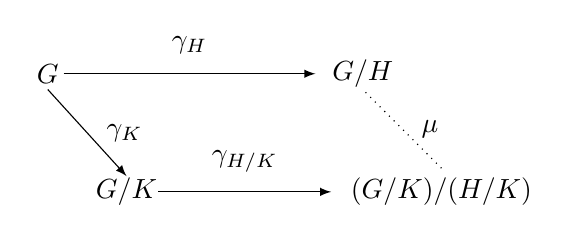
\begin{tikzpicture}
		\draw (0,1.5) node {$G$};
		\draw (1,0) node {$G/K$};
		\draw (5,0) node {$(G/K)/(H/K)$};
		\draw (4,1.5) node {$G/H$};
		\draw[-latex] (0,1.3) -- node(e1)[label=right:$\gamma_K$]{} (1,0.2);
		\draw[-latex] (0.2,1.5) -- node(e2)[label=above:$\gamma_H$]{} (3.4,1.5);
		\draw[-latex] (1.4,0) -- node(e3)[label=above:$\gamma_{H/K}$]{} (3.6,0);
		\draw[dotted] (5,0.3) -- node(e4)[label=right:$\mu$]{} (4,1.3);
	\end{tikzpicture}
	\caption{Third Isomorphism Theorem}
\end{figure}
\end{frame}

\begin{frame}
\frametitle{Third Isomorphism Theorem}
	\begin{figure}
		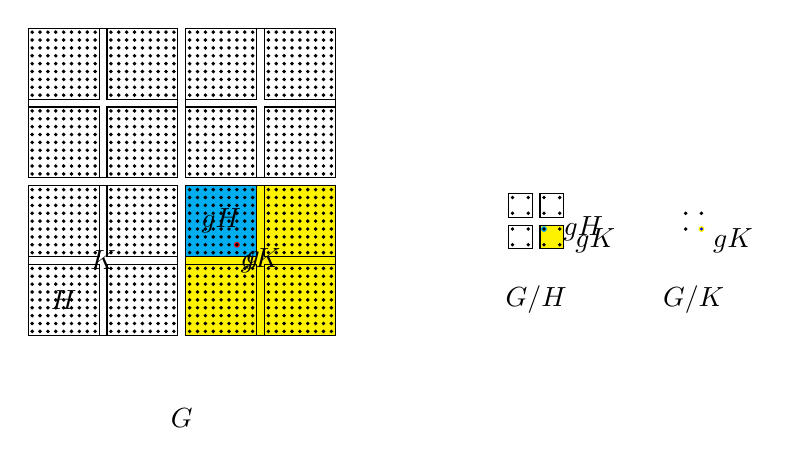
\begin{tikzpicture}
		\draw<3>[yellow,fill = yellow] (6.55,1.15) rectangle (6.85,1.45);
		\draw<3>[yellow,fill = yellow] (2.05,0.05) rectangle (3.95,1.95);
		\draw<2->[cyan,fill = cyan] (6.6,1.4) circle[radius=0.03];
		\draw<2->[cyan,fill = cyan] (2.05,1.05) rectangle (2.95,1.95);
		\draw[red,fill = red] (2.7,1.2) circle[radius=0.03];

		\draw node at (2,-1) {$G$};
		\draw<1> node at (2.9,1) {$g$};
		\draw<2-> node at (6.5,0.5) {$G/H$};
		\draw<2> node at (0.5,0.5) {$H$};
		\draw<2> node at (2.5,1.5) {$gH$};
		\draw<2> node at (7.1,1.4) {$gH$};
		\draw<3> node at (1,1) {$K$};
		\draw<3> node at (8.5,0.5) {$G/K$};
		\draw<3> node at (9,1.25) {$gK$};
		\draw<3> node at (7.25,1.25) {$gK$};
		\draw<3> node at (3,1) {$gK$};
		%Group G
		%\draw<1-1> (0,0) rectangle (4,4);
		%coset division G/N
		\foreach \ii in {0,...,3}{
			\foreach \jj in {0,...,3}{
				\draw<2> (0.05+\ii,0.05+\jj) rectangle (0.95+\ii,0.95+\jj);
			}}
		%coset division G/L
		\draw<3> (0.05,0.05) rectangle (1.95,1.95);
		\draw<3> (0.05,2.05) rectangle (1.95,3.95);
		\draw<3> (2.05,0.05) rectangle (3.95,1.95);
		\draw<3> (2.05,2.05) rectangle (3.95,3.95);
		%elements of G
		\foreach \ii in {0,...,3}{
			\foreach \jj in {0,...,3}{
				\foreach \kk in {1,...,9}{
					\foreach \ll in {1,...,9}{
						\draw<1->[black,fill=black] (\ii.\kk,\jj.\ll) circle[radius=0.015];
			}}}}
		%Group G/N
		%\draw<4-4> (6,1) rectangle (7,2);
		%\coset division G/L
		\draw<3> (6.15,1.15) rectangle (6.45,1.45);
		\draw<3> (6.15,1.55) rectangle (6.45,1.85);
		\draw<3> (6.55,1.15) rectangle (6.85,1.45);
		\draw<3> (6.55,1.55) rectangle (6.85,1.85);
		%elements of G/N
		\foreach \ii in {2,4,6,8}{
			\foreach \jj in {2,4,6,8}{
				\draw<2->[black,fill=black] (6.\ii,1.\jj) circle[radius=0.015];
			}}
		\draw<3->[black,fill=black] (8.4,1.4) circle[radius=0.015];
		\draw<3->[black,fill=black] (8.4,1.6) circle[radius=0.015];
		\draw<3->[yellow,fill=yellow] (8.6,1.4) circle[radius=0.03];
		\draw<3->[blue,fill=blue] (8.6,1.4) circle[radius=0.01];
		\draw<3->[black,fill=black] (8.6,1.6) circle[radius=0.015];
		\end{tikzpicture}
	\end{figure}
\end{frame}
